\section{CamilleX Overview}
\label{sec:overview}

The CamilleX provides new CamilleX constructs (XMachines and XContexts) which are text files which are automatically translated into the corresponding Rodin Event-B constructs (i.e., Machine and Context) accordingly.  Facility for translating from Rodin Event-B components to CamilleX components can be invoked manually. The overall process can be seen in Figure~\ref{fig:overview}.
\begin{figure}[!htbp]
  \centering
  \ifdef{PLASTEX}
  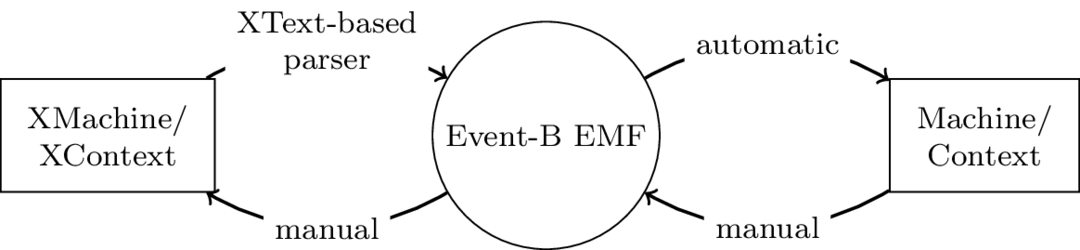
\includegraphics{figures/tikz-overview.png}
  \endif
  \ifdef{PANDOC}
  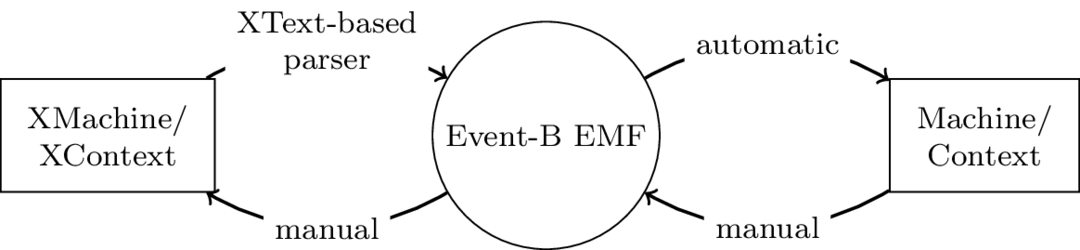
\includegraphics{figures/tikz-overview.png}
  \endif
  \ifdef{LATEX}
  \documentclass[convert={density=300,size=1080x800,outext=.png}]{standalone}

\usepackage{tikz}
\usepackage{tikz-eventB}
\usetikzlibrary{fit}
\usetikzlibrary{positioning}
\usetikzlibrary{arrows}

\begin{document}
\begin{tikzpicture}
  \footnotesize
  \tikzMch[Rodin]{0}{0}{
    Machine/
    \\
    Context
  }
  \tikzMch[XEventB]{-8}{0}{%
    XMachine/
    \\
    XContext
  }

  \node[draw, circle] (EMF) at (-4, 0) {Event-B EMF};
  \path [->, thick] (XEventB) edge [bend left]  node[fill=white, align = center]{XText-based\\parser} (EMF);
  \path [->, thick] (EMF) edge [bend left] node[fill=white]{automatic} (Rodin);
  
  \path [->, thick] (Rodin) edge [bend left]  node[fill=white]{manual} (EMF);
  \path [->, thick] (EMF) edge [bend left] node[fill=white]{manual} (XEventB);
\end{tikzpicture}
\end{document}

  \endif
  \caption{Overview of CamilleX and Rodin Event-B Constructs}
  \label{fig:overview}
\end{figure}

%%% Local Variables:
%%% mode: latex
%%% TeX-master: "user_manual"
%%% End:
